\documentclass[aspectratio=169]{beamer}
\usepackage{amsmath}
\usepackage{tikz}
\usepackage{xcolor}
\usetikzlibrary{arrows}
\usetikzlibrary{calc}

\usetheme{Pittsburgh}
\setbeamercolor{background canvas}{bg=black}
\setbeamercolor{normal text}{fg=white}
\setbeamertemplate{navigation symbols}{}
\usefonttheme[onlymath]{serif}

% For every picture that defines or uses external nodes, you'll have to
% apply the 'remember picture' style. To avoid some typing, we'll apply
% the style to all pictures.
\tikzstyle{every picture}+=[remember picture]

% Stop tikz typesetting math in inline mode.
\everymath{\displaystyle}

\newcommand{\defaulttrans}{\transdissolve[duration=0.25]}

\colorlet{hi1}{blue!50!white}
\colorlet{hi2}{green!40!white}
\colorlet{hi3}{red!65!white}

\begin{document}

\frame{
    % Empty frame
}

% 1. Consider some point vector and two basis vectors e_x, e_y
% 2. We can resolve the point
% 3. But what about some other co-ordinate system?
% 4. We can also resolve onto this
% 5. Which is right?
\frame{\centering
    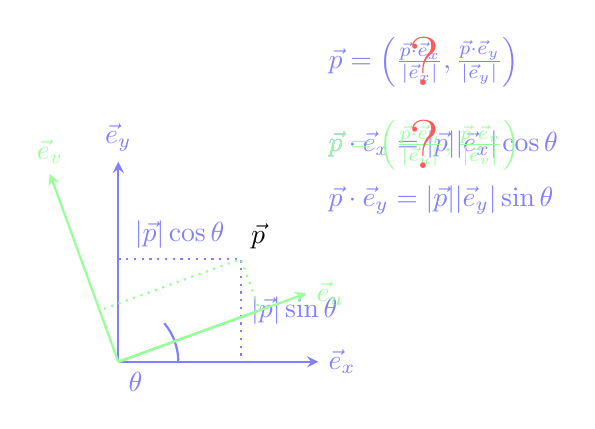
\begin{tikzpicture}[draw=white,thick,x=1in,y=1in]
        \coordinate (O) at (0,0);
        \coordinate (P) at ($ (O) + (xy polar cs:angle=40, radius=0.8) $);
        \coordinate (X) at ($ (O) + (xy polar cs:angle=0, radius=1) $);
        \coordinate (Y) at ($ (O) + (xy polar cs:angle=90, radius=1) $);
        \coordinate (U) at ($ (O) + (xy polar cs:angle=20, radius=1) $);
        \coordinate (V) at ($ (O) + (xy polar cs:angle=110, radius=1) $);
        \draw[-stealth] (O) -- (P) node[above right] {$\vec{p}$};
        \begin{scope}[draw=hi1,fill=hi1,every node/.style={text=hi1}]
            \draw[-stealth] (O) -- (X) node[right] {$\vec{e}_x$};
            \draw[-stealth] (O) -- (Y) node[above] {$\vec{e}_y$};
        \end{scope}
        \uncover<2->{
            \begin{scope}[draw=hi1,fill=hi1,every node/.style={text=hi1}]
                \draw (O) -- ($(O)!(P)!(X)$);
                \draw (O) -- ($(O)!(P)!(Y)$);
                \draw[dotted] ($(O)!(P)!(Y)$) -- node (px) {} (P) -- node (py) {} ($(O)!(P)!(X)$);
                \uncover<2> {
                    \path (px) node[above] {$|\vec{p}| \cos\theta$};
                    \path (py) node[right] {$|\vec{p}| \sin\theta$};
                    \draw (O) +(0:0.3) arc [radius=0.3, start angle=0, end angle=40];
                    \path (O) node[below right] {$\theta$};
                }
                \path (1,1.5) node[right] (def1)
                {$\vec{p} = \left(\frac{\vec{p}\cdot\vec{e}_x}{|\vec{e}_x|},\frac{\vec{p}\cdot\vec{e}_y}{|\vec{e}_y|}\right)$};
                \only<2>{
                    \path (1,1.5) ++ (0, -3em) node[right]
                    {$\vec{p}\cdot\vec{e}_x = |\vec{p}||\vec{e}_x| \cos\theta$};
                    \path (1,1.5) ++ (0, -5em) node[right]
                    {$\vec{p}\cdot\vec{e}_y = |\vec{p}||\vec{e}_y| \sin\theta$};
                }
            \end{scope}
        }
        \uncover<3->{
            \begin{scope}[draw=hi2,fill=hi2,every node/.style={text=hi2}]
                \draw[-stealth] (O) -- (U) node[right] {$\vec{e}_u$};
                \draw[-stealth] (O) -- (V) node[above] {$\vec{e}_v$};
            \end{scope}
        }
        \uncover<4->{
            \begin{scope}[draw=hi2,fill=hi2,every node/.style={text=hi2}]
                \draw (O) -- ($(O)!(P)!(U)$);
                \draw (O) -- ($(O)!(P)!(U)$);
                \draw[dotted] (O) -- ($(O)!(P)!(U)$) -- (P) -- ($(O)!(P)!(V)$) -- (O);
            \end{scope}
            \path (1,1.5) ++ (0, -3em) node[right] (def2)
            {$\color{hi2} \vec{p} = \left(\frac{\vec{p}\cdot\vec{e}_u}{|\vec{e}_u|},\frac{\vec{p}\cdot\vec{e}_v}{|\vec{e}_v|}\right)$};
        }
        \uncover<5->{
            \path (def1) node[text=hi3] {\Huge ?};
            \path (def2) node[text=hi3] {\Huge ?};
        }
    \end{tikzpicture}\\
}

% 1. Look at the dot-product
% 2. We go across ..
% 3. .. and then down
% 4. Pairs of numbers correspond (1)
% 5. Pairs of numbers correspond (2)
% 6. The important thing is that the number 'K' matches
\frame{\[
    \tikz[baseline]{ \node (x) { 
        $ \begin{bmatrix} \color<4->{hi1}{x_1} & \color<5->{hi2}{x_2} & \cdots & x_{\color<6->{hi3} K} \end{bmatrix} $
    }; }
    \tikz[baseline]{ \node (y) { 
        $ \begin{bmatrix} \color<4->{hi1}{y_1} \\ \color<5->{hi2}y_2 \\ \vdots \\ y_{\color<6->{hi3} K} \end{bmatrix} $
    }; }
    = { \color<4->{hi1} x_1 y_1} + { \color<5->{hi2} x_2 y_2} + \cdots + x_{\color<6->{hi3} K} y_{\color<6->{hi3} K}
\]

\begin{tikzpicture}[overlay, draw=hi3]
    \path[->]<2-> (x.south west) edge (x.south east);
    \path[->]<3-> (y.north east) edge (y.south east);
\end{tikzpicture}
}

% 1. If we write this using a short-hand for row- and column- vectors
% 2. We have the following sizes
\frame{\[
    \begin{array}{cccc}
    \begin{bmatrix} \mbox{\ ---} & \vec{x} & \mbox{---\ } \end{bmatrix}&
    \begin{bmatrix} | \\[0.5ex] \vec{y} \\[0.5ex] | \end{bmatrix}&
    =&
    \vec{x} \cdot \vec{y} \\
    \uncover<2->{ \\ 1 \times K & K \times 1 & \rightarrow & 1 \times 1 }
    \end{array}
\]}

% 1. If we put an index on the 'x' vector
% 2. We can stack a row below it
% 3. And again
% 4. We end up with these sizes
\frame{\[
    \begin{array}{cccc}
    \begin{bmatrix}
        \mbox{\ ---} & \vec{x}_1 & \mbox{---\ }
        \only<2->{ \\ \mbox{\ ---} & \vec{x}_2 & \mbox{---\ } }
        \only<3->{ \\ \mbox{\ ---} & \vec{x}_3 & \mbox{---\ } }
    \end{bmatrix} &
    \begin{bmatrix} | \\[0.5ex] \vec{y} \\[0.5ex] | \end{bmatrix} &
    = & 
    \begin{bmatrix}
        \vec{x}_1 \cdot \vec{y}
        \only<2->{ \\ \vec{x}_2 \cdot \vec{y}}
        \only<3->{ \\ \vec{x}_3 \cdot \vec{y}}
    \end{bmatrix} \\
    \uncover<4->{ \\ 3 \times K & K \times 1 & \rightarrow & 3 \times 1 }
    \end{array}
\]}

% 1. We can put an index on 'y' too
% 2. And add a column
% 3. And another
% 4. Now a row of x
% 5. And another
% 6. Notice how each pair of row and columns has an entry on the right-hand side? (1)
% 7. Notice how each pair of row and columns has an entry on the right-hand side? (2)
% 8. We end up with these sizes
\frame{\[
    \begin{array}{cccc}
    \begin{bmatrix}
        \color<7>{hi1} \mbox{\ ---} & \color<7>{hi1} \vec{x}_1 & \color<7>{hi1} \mbox{---\ } 
        \only<4->{ \\ \mbox{\ ---} & \vec{x}_2 & \mbox{---\ } }
        \only<5->{ \\ \color<6>{hi1} \mbox{\ ---} & \color<6>{hi1} \vec{x}_3 & \color<6>{hi1} \mbox{---\ } }
    \end{bmatrix}&
    \begin{bmatrix}
        | \only<2->{& \color<6>{hi1} \color<7>{hi1} |} \only<3->{& |} \\[0.5ex]
        \vec{y}_1 \only<2->{& \color<6>{hi1} \color<7>{hi1} \vec{y}_2} \only<3->{& \vec{y}_3} \\[0.5ex]
        | \only<2->{& \color<6>{hi1} \color<7>{hi1} |} \only<3->{& |} \end{bmatrix}&
    =&
    \begin{bmatrix}
        \vec{x}_1 \cdot \vec{y}_1
        \only<2->{& \color<7>{hi1} \vec{x}_1 \cdot \vec{y}_2}
        \only<3->{& \vec{x}_1 \cdot \vec{y}_3}
        \only<4->{\\
            \vec{x}_2 \cdot \vec{y}_1 & \vec{x}_2 \cdot \vec{y}_2 & \vec{x}_2 \cdot \vec{y}_3
        }
        \only<5->{\\
            \vec{x}_3 \cdot \vec{y}_1 & \color<6>{hi1} \vec{x}_3 \cdot \vec{y}_2 & \vec{x}_3 \cdot \vec{y}_3
        }
    \end{bmatrix} \\
    \uncover<8->{ \\ 3 \times K & K \times 3 & \rightarrow & 3 \times 3 }
    \end{array}
\]}

% 1. This is the full version of the matrix product
% 2. And here are the sizes
\frame<-2>[label=matrix-product]{\[
    \begin{array}{cccc}
    \begin{bmatrix}
        \mbox{\ ---} &  \vec{x}_1 & \mbox{---\ } \\
        \mbox{\ ---} &  \vec{x}_2 & \mbox{---\ } \\
        & \vdots & \\
        \mbox{\ ---} &  \vec{x}_M & \mbox{---\ }
    \end{bmatrix}&
    \begin{bmatrix}
        | & | & & | \\
        \vec{y}_1 & \vec{y}_2 & \cdots & \vec{y}_N \\
        | & | & & |
    \end{bmatrix}&
    =&
    \begin{bmatrix}
        \vec{x}_1 \cdot \vec{y}_1 & \vec{x}_1 \cdot \vec{y}_2 & \cdots & \vec{x}_1 \cdot \vec{y}_N \\
        \vec{x}_2 \cdot \vec{y}_1 & \vec{x}_2 \cdot \vec{y}_2 & \cdots & \vec{x}_2 \cdot \vec{y}_N \\
        \vdots & \vdots & \ddots & \vdots \\
        \vec{x}_M \cdot \vec{y}_1 & \vec{x}_M \cdot \vec{y}_2 & \cdots & \vec{x}_M \cdot \vec{y}_N
    \end{bmatrix}\\
    \uncover<2->{ \\ \color<4>{hi1} M \times {\color<5->{hi1} K} & \color<4>{hi1} {\color<5->{hi1} K} \times N & \color<4>{hi1} \rightarrow & \color<4>{hi1} M \times N }
    \end{array}
\]}

\frame{ \centering
Matrices are just horizontal and vertical stacks of {\color{hi1} vectors}. \\[1em]
\uncover<2->{They are \emph{not} rectangles full of numbers. \\[1em]}
}

\frame{ \centering
    {\color{hi1} Matrix products} are just {\color{hi2} dot-products} between rows and columns. \\
}

% 3. Look at this again
% 4. The bottom bit is important. It will tell you if your matrix product will work
% 5. As long as the inner sizes match, everything will work
\againframe<3->{matrix-product}

\end{document}

% you may need to set makeprg=pdflatex\ -interaction=nonstopmode\ % 
